\documentclass{article} % say
\usepackage{tikz}
\usepackage[T1]{fontenc}
\usepackage{libertine,textcomp}%% Only as example for the romans/sans fonts
\usepackage[scaled=0.85]{beramono}
\usetikzlibrary{calc,arrows,decorations.pathmorphing,backgrounds,fit,positioning,datavisualization}


\begin{document}
%\tikzset{pop1/.style={blue!40},pop2/.style={red!40}}
\centering

    
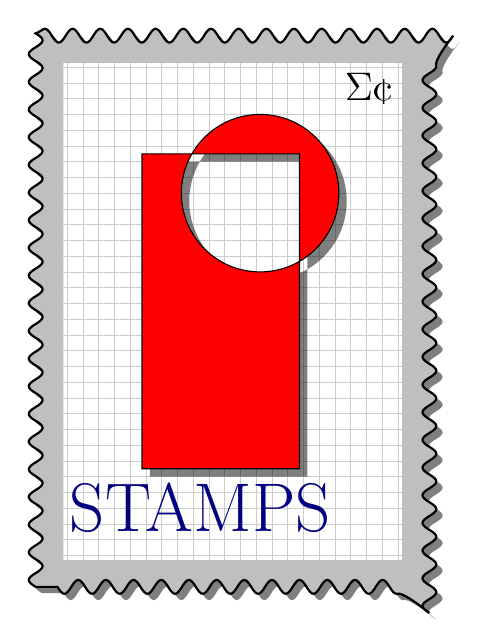
\begin{tikzpicture}[scale=.5]


% Outer edge of STAMP
\filldraw
[preaction={fill=black,opacity=.5,
                transform canvas={xshift=.8mm,yshift=-.8mm}}]
[fill=black!25,decorate,decoration={coil,aspect=0},thick] (0,0) -- (0,14) -- (10,14) -- (10,0) -- cycle;

% Inner edge of STAMP
\begin{scope}
\clip (.7,.7) rectangle (9.3,13.3);
\fill[white] (0,0) rectangle (10,14);

\draw[step=.4cm,black!20,very thin] (0,0) grid (10,14);

\draw
    [preaction={fill=black,opacity=.5,
                transform canvas={xshift=1mm,yshift=-1mm}}]
    [fill=red] (2.7,3) rectangle +(4,8)
               (5.7,10) circle (20mm);
               
\node[font=\large,inner sep=0mm,left=0mm,color=blue!50!black] at (7.5, 2) {{\Huge STAMPS}};

%\fill[orange!20] (1,1) rectangle (9,13);

\node[anchor=north east] at (9.3,13.3) {{\Large $\Sigma$\textcent}};
\end{scope}


\end{tikzpicture}  

\end{document}